\chapter{Teoria della complessità} \label{ch:capitolo9}
\subsection{Costo della computazione}
\textbf{Problema}\\
Cosa si può calcolare con un costo ragionevole?\\\\
\textbf{Osservazione}\\
Il costo dipende dall’algoritmo\\\\
\textbf{Esempio}\\
Vogliamo determinare il valore del polinomio
\begin{center}
    $x^7 + 5x^6 + 2x^4 + 12x^3 + 5x^2 + 2x + 21$
\end{center}
per certi input x . Quante moltiplicazioni servono?
\begin{itemize}
    \item per ciascun monomio, nell’ordine, 6,6,4,3,2,1, totale: 22
    
    \item se calcolo prima tute le potenze di x (6 moltiplicazioni), per ciascun monomio, nell’ordine, 0,1,1,1,1,1, totale: 11
    
    \item se scrivo il polinomio nella forma
\end{itemize}
\begin{center}
    $(((((x + 5)x^2 + 2)x + 12)x + 5)x + 2)x + 21$
\end{center}
\newpage
\textbf{Esempio}\\
Per calcolare il massimo comun divisore di due interi positivi a e b si può:
\begin{itemize}
    \item decomporre a e b in fattori primi
    
    \item selezionare i fattori primi comuni, con il minimo esponente
\end{itemize}
oppure usare l’algoritmo di Euclide:\\
\begin{figure}[htp]
    \centering
    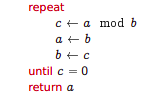
\includegraphics[scale=0.9]{tesi_stile/img/f1cap9.png}
\end{figure}
\newpage
\begin{figure}[htp]
    \centering
    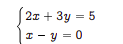
\includegraphics[scale=0.9]{tesi_stile/img/f2cap9.png}
\end{figure}
Per risolvere un sistema lineare si può utilizzare il metodo di Cramer:\\
\begin{figure}[htp]
    \centering
    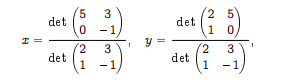
\includegraphics[scale=0.9]{tesi_stile/img/f3cap9.png}
\end{figure}\\
oppure ridurre il sistema in forma triangolare:\\
\begin{figure}[htp]
    \centering
    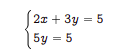
\includegraphics[scale=0.9]{tesi_stile/img/f4cap9.png}
\end{figure}
\newpage
\subsection{Teoria della complessità}
\textbf{Quale risorsa misurare?}\\
Tempo, memoria, energia,...\\\\
\textbf{Quale modello di calcolo?}\\
Macchina di Turing, altri?.\\\\
\textbf{Quali problemi considerare?}\\
\begin{itemize}
    \item Problemi di \textbf{decisione}
    
dato $S \subseteq A*$, decidere per ogni input $w \in A*$ se $w \in S$.

    \item Problemi di \textbf{computazione}
    
Data $f : A* \mapsto A*$ calcolare, per ogni input $w \in A*$ , f(w)

    \item problemi di ottimizzazione
    
    \item problemi di ricerca

\end{itemize}
\subsection{Teoria della complessità2}
\textbf{Che risultati cerchiamo?}\\
Vogliamo conoscere il costo minimo per risolvere un problema (non un particolare algoritmo). Ci aspettiamo
\begin{itemize}
    \item Risultati negativi
    
    il problema non si può risolvere senza...
    
    \item Risultati di confronto
    
    per risolvere il problema S servono almeno le stesse risorse necessarie a risolvere il problema T
\end{itemize}
\subsection{Come misurare la complessità}
Vogliamo valutare il costo della computazione in funzione della complessità dell’input.
Sia S un problema (di decisione) sull’alfabeto A. Consideriamo una funzione $f : N \mapsto N$ calcolata come segue:
\begin{itemize}
    \item per ogni $n \in N$ consideriamo tutti gli input di lunghezza minore o uguale a n e il costo delle relative computazioni (escludendo quelle che non terminano)
    
    \item f(n) restituirà il massimo costo di tali computazioni
\end{itemize}
\textbf{Proprietà delle funzioni costo}
\begin{itemize}
    \item una funzione costo è definita per n $>= n_0$, con $n_0 \in N$ opportuno
    
    \item non decrescente
    
    \item non limitata
\end{itemize}
\textbf{Esempi}\\
$n, n^2, n^k, 2^n, 2^{2n}, |\log_2 n|$, polinomi a coefficienti non negativi.\\\\
\newpage
\textbf{Esempio}\\
Quante divisioni servono per l’algoritmo Euclideo del MCD?\\
Supponiamo a $>=$ b e calcoliamo MCD(a, b).\\
\begin{figure}[htp]
    \centering
    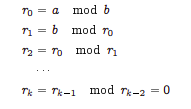
\includegraphics[scale=0.9]{tesi_stile/img/f5cap9.png}
\end{figure}\\
Pertanto.
\begin{figure}[htp]
    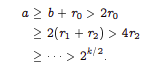
\includegraphics[scale=0.9]{tesi_stile/img/f6cap9.png}
\end{figure}\\
Ne segue\\
\begin{center}
    $k < 2\log_2 a$
\end{center}
Pertanto:\\
Il numero di divisioni necessario per calcolare MCD(a, b) è linearmente limitato dalla lunghezza della rappresentazione binaria di a.\\\\
\textbf{Osservazione}\\
Per le funzioni numeriche, la complessità dell’input è misurata dal numero di bit (o cifre decimali) necessaria per rappresentarlo:
\begin{center}
    $1 + |\log_2(n)|$
\end{center}
\newpage
\subsection{Complessità temporale}
\textbf{Definizione}\\
Sia M una macchina di Turing. Si dice complessità temporale di M la funzione $c_M : N \mapsto N$ definita come segue:\\
per ogni $n \in N$, $c_M (n)$ è il massimo numero di passi di una computazione convergente di M su un input di lunghezza minore o uguale a n.\\\\
\textbf{Osservazione}\\
La funzione $c_M$ è definita per $n >= n_0$ con $n_0 \in N$, non decrescente e non limitata (purchè $c_M$ abbia un dominio infinito e M esamini l’intero input su ogni computazione).
\subsection{La classe P}
\textbf{Definizione}\\
Denotiamo con P la classe dei problemi S accettati da una macchina di Turing M tale che $c_M (n) = O(n^k)$ per qualche intero positivo k.\\\\
\textbf{Osservazione}\\
Se $S \in P$, allora c’è una macchina di Turing che, per ogni input w di lunghezza n, si comporta nel modo seguente:
\begin{itemize}
    \item se $w \in S$, allora M accetta w in al più $cl(w)^k$ passi (con c, k costanti positive fissate)
    
    \item se $w \notin S$, allora $M \uparrow w$
\end{itemize}
In realtà, c’è anche una macchina di Turing M'
che decide S con $c_{M'}(n) = O(n^k)$.
\newpage
\subsection{Tesi di Edmonds-Cook-Karp}
\begin{figure}[htp]
    \centering
    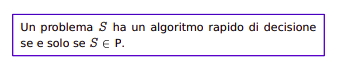
\includegraphics[scale=0.9]{tesi_stile/img/f10cap9.png}
\end{figure}
\textbf{Osservazione}\\
Riferita ai problemi, non agli algoritmi.\\\\
\textbf{Osservazione}\\
La definizione di P è robusta:\\
se esiste un algoritmo che decide S e richiede l’esecuzione di $O(n^k)$ istruzioni (comunque specificate, purchè simulabili da una macchina di Turing in tempo polinomiale), allora $s \in P$.




